\documentclass[12pt]{article}
\usepackage[utf8]{inputenc}
\usepackage{float}
\usepackage{amsmath}


\usepackage[hmargin=3cm,vmargin=6.0cm]{geometry}
%\topmargin=0cm
\topmargin=-2cm
\addtolength{\textheight}{6.5cm}
\addtolength{\textwidth}{2.0cm}
%\setlength{\leftmargin}{-5cm}
\setlength{\oddsidemargin}{0.0cm}
\setlength{\evensidemargin}{0.0cm}

%misc libraries goes here
\usepackage{tikz}
\usetikzlibrary{automata,positioning}

\begin{document}

\section*{Student Information } 
%Write your full name and id number between the colon and newline
%Put one empty space character after colon and before newline
Full Name : Bilal Özlü \\
Id Number : 1942614 \\

% Write your answers below the section tags
\section*{Answer 1}

\subsection*{a.}
$\lbrace$ x$^a$y$^a$z$^b$ : a,b $\geq$ 0 $\rbrace$  $\cup$  $\lbrace$ x$^a$y$^b$z$^a$ : a,b $\geq$ 0 $\rbrace$ \\

\subsection*{b.}
U = (x,y)* $\char36$V (x,y)* : left and right side of $\char36$V are reverse of each other. \\
V = (x,y)* \\
So the language is: UV : $\underbrace{(x,y)}$* $\char36$(x,y)* $\underbrace{(x,y)}$* (x,y)* \\
.$\hspace{138pt}$w$\hspace{68pt}$w$^R$ \\

\subsection*{c.}
The regular expression is: x(x$^9$)* + ((z,y)(z,y))* \\

\section*{Answer 2}

\subsection*{a.}
Assume that L$_1$ is a context free language. \\
Since L$_1$ is infinite, we can apply Pumping Lemma. \\
Let a = 2$^m$1$^m$. Then, L$_1$ = aa$^R$2$^{|a|}$ = 2$^m$1$^m$1$^m$2$^m$2$^{2m}$ \\
By Pumping Lemma, a can be decomposed as a = uvxyz with $\vert$vxz$\vert$ $\leq$ m and $\vert$vy$\vert$ $\geq$ 1 such that uv$^i$xy$^i$z $\in$L$_1$ for i $\geq$ 0. \\
\\
$\bullet$Case 1 \\
for i = 0 \\
$\underbrace{22...211...}$ $\underbrace{11...122...2}$ \\
.$\hspace{14pt}$uvxy$ \hspace{42pt}$z \\
$\vert$a$\vert$ = 2m - $\vert$vy$\vert$ is less than $\vert$ a$^R$ $\vert$, so uv$^0$xy$^0$z $\notin$ L$_1$ \\
$\bullet$Case 2 \\
for i = 0 \\
$\underbrace{22...211...1}$ $\underbrace{11...122...}$ $\underbrace{22...2}$ \\
.$\hspace{18pt}$u$\hspace{45pt}$vxy$\hspace{30pt}$z \\
$\vert$ a$^R$ $\vert$ = 2m - $\vert$vy$\vert$ is less than $\vert$a$\vert$, so uv$^0$xy$^0$z $\notin$ L$_1$ \\
$\bullet$Case 3 \\
for i=0 \\
$\underbrace{22...211...1122...2}$ $\underbrace{22...2}$ \\
.$\hspace{36pt}$u$ \hspace{48pt}$vxyz \\
$\vert$ 2$^{|a|}$ $\vert$ = 2m - $\vert$vy$\vert$ is less than $\vert$a$\vert$. So, uv$^0$xy$^0$z $\notin$ L$_1$ \\
$\bullet$Case 4 \\
for i = 0 \\
$\underbrace{22...1}$ $\underbrace{11...1}$ $\underbrace{122...22...2}$\\
.$\hspace{8pt}$u$\hspace{20pt}$vxy$\hspace{30pt}$z \\
$\vert$ a$\vert$ 2$^{|a|}$ $\vert$ $\vert$ = 4m - $\vert$vy$\vert$ \\
(4m - $\vert$vy$\vert$)/2 $<$ $\vert$ 2$^{|a|}$ $\vert$ = 2m. So, uv$^0$xy$^0$z $\notin$ L$_1$ \\
$\bullet$Case 5 \\
for i = 0 \\
$\underbrace{22...11...12}$ $\underbrace{22...2}$ $\underbrace{22...2}$ \\
.$\hspace{24pt}$u$\hspace{34pt}$vxy$\hspace{20pt}$z \\
$\vert$ a$^R$2$^{|a|}$ $\vert$ = 4m - $\vert$vy$\vert$ \\
(4m - $\vert$vy$\vert$)/2 $<$ $\vert$a$\vert$ = 2m. So, uv$^0$xy$^0$z $\notin$ L$_1$ \\
Contradiction. Then, this assumption is false. \\
Hence, L$_1$ is not context-free. \\

\subsection*{b.}
L$_2$ is a CFL. \\
$\bullet$A is context free. \\
S $\rightarrow$ xSz $\vert$ T \\
T $\rightarrow$ yTz $\vert$ $\varepsilon$ \\
$\bullet$B is a regular language. \\
S $\rightarrow$ XY \\
X $\rightarrow$ x $\vert$ xx $\vert$ xxx $\vert$... $\vert$ x$^{100}$ $\vert$ $\varepsilon$ \\
Y $\rightarrow$ y $\vert$ yy $\vert$ yyy $\vert$... $\vert$ y$^{100}$ $\vert$ $\varepsilon$ \\
Note that if B is a RL, also $\overline{B}$ is a RL. \\
L$_2$ = A $\setminus$ B = A $\cap$ $\overline{B}$ is context-free. \\
Intersection of a CFL and a RL is a context-free language because we can construct a new NPDA machine that accepts the NPDA of that context free language and the DFA of that regular language. \\

\subsection*{c.}
Assume that L$_3$ is a context free language. \\
Since L$_3$ is infinite, we can apply Pumping Lemma. \\
Pick a string w = a$^k$b$^k$c$^{k^2}$ , w $\in$ L$_3$. \\
By Pumping Lemma w can be decomposed as w = uvxyz with $\vert$vxz$\vert$ $\leq$ k \\
and $\vert$vy$\vert$ $\geq$ 1 such that uv$^i$xy$^i$z $\in$L$_3$ for i $\geq$ 0. \\
Now, We will examine all the possible locations of string vxz in w. \\
$\bullet$Case 1 \\
for i=0 \\
$\underbrace{aaa...a}$ $\underbrace{aabb...bcc...c}$ \\
.$\hspace{2pt}$uvxy$ \hspace{38pt}$z \\
uv$^0$xy$^0$z = a$^{k-|vy|}$b$^k$c$^{k^2}$ $\notin$ L$_3$ \\
$\bullet$Case 2 \\
for i=0 \\
$\underbrace{aaa...a}$ $\underbrace{ab}$ $\underbrace{b...b}$ $\underbrace{bcc...b}$ \\
.$\hspace{10pt}$uv$\hspace{20pt}$x$\hspace{20pt}$y$\hspace{22pt}$z \\
uv$^0$xy$^0$z = a$^{k-|v|}$b$^{k-|y|}$c$^{k^2}$ $\notin$ L$_3$ \\
$\bullet$Case 3 \\
for i=0 \\
$\underbrace{aaa...ab}$ $\underbrace{b...b}$ $\underbrace{bcc...c}$ \\
.$\hspace{12pt}$u$\hspace{23pt}$vxy$\hspace{20pt}$z \\
uv$^0$xy$^0$z = a$^k$b$^{k-|vy|}$c$^{k^2}$ $\notin$ L$_3$ \\
$\bullet$Case 4 \\
for i=0 \\
$\underbrace{aaa...ab}$ $\underbrace{b...b}$ $\underbrace{bc}$ $\underbrace{cc...c}$ \\
.$\hspace{14pt}$u$\hspace{27pt}$v$\hspace{20pt}$x$\hspace{18pt}$yz \\
uv$^0$xy$^0$z = a$^k$b$^{k-|v|}$c$^{k^2 - |y|}$ $\notin$ L$_3$ \\
$\bullet$Case 5 \\
for i=0 \\
$\underbrace{aaa...abb...bc}$ $\underbrace{c...c}$ \\
.$\hspace{25pt}$u$\hspace{30pt}$vxyz \\
uv$^0$xy$^0$z = a$^k$b$^k$c$^{k^2 - |vy|}$ $\notin$ L$_3$ \\
$\bullet$Case 6 \\
v or y containing "ab" or "bc" \\
If i$>$0, uv$^i$xy$^i$z would be a…ab…bc…cb…c or a…ab…ba…ab…b…c…c. And it would not be in L$_3$. \\
There are no other cases to examine, and we got contradiction in all cases above. \\
So, L$_3$ is not context-free. \\

\subsection*{d.}
L$_4$ = $\overline{L}$ = (1,2)* - L  \\
L$_4$ = $\lbrace$(1,2)* - 1*2*$\rbrace$ $\cup$ $\lbrace$ 1$^n$2$^m$ : n$>$m $\rbrace$ $\cup$ $\lbrace$ 1$^n$2$^m$ : m$>$2n $\rbrace$ \\
If each of the three parts of L$_4$ is context-free, we can see that L$_4$ is context-free, since union operator is closed for CFLs. \\
$\bullet$ $\lbrace$(1,2)* - 1*2*$\rbrace$ is a regular language. Because (1,2)* and 1*2* are regular clearly and set difference is closed for RLs. And also every RL is a CFL. \\
$\bullet$ $\lbrace$ 1$^n$2$^m$ : n$>$m $\rbrace$ is a context free language. \\
S $\rightarrow$ 1A \\
A $\rightarrow$ 1A $\vert$ 1A2 $\vert$ $\varepsilon$ \\
$\bullet$ $\lbrace$ 1$^n$2$^m$ : m$>$2n $\rbrace$ is a context free language. \\
S $\rightarrow$ A2 \\
A $\rightarrow$ A2 $\vert$ 1A22 $\vert$ $\varepsilon$ \\
So, L$_4$ is context-free. \\

\section*{Answer 3}

\subsection*{a.}
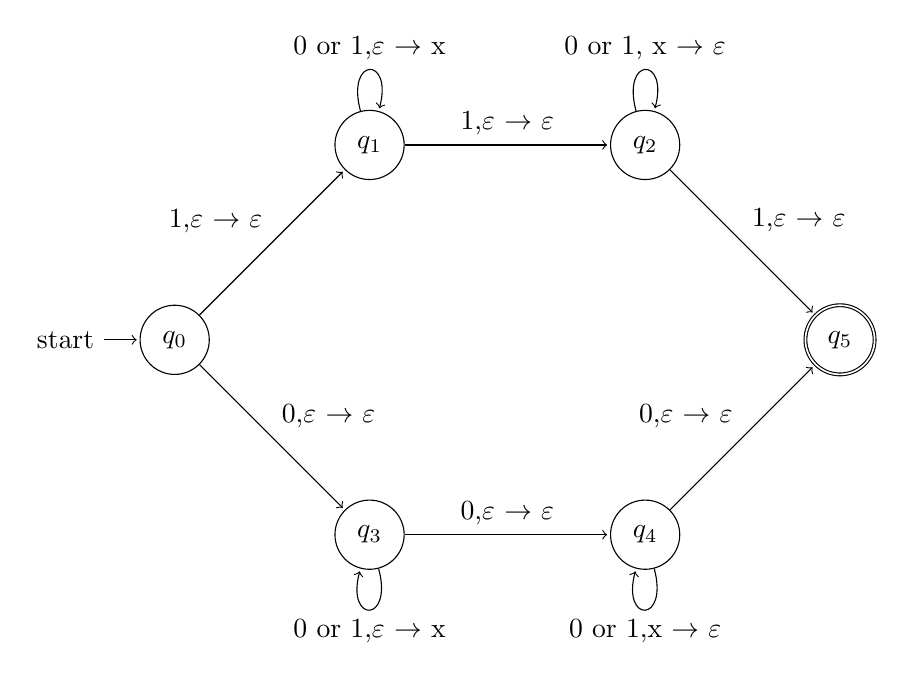
\begin{tikzpicture}[shorten >=1pt,node distance=3.5cm,on grid,auto]
\node[state, initial] (q_0) {$q_0$};
\node[state] (q_1) [above right=of q_0] {$q_1$};
\node[state] (q_2) [right=of q_1] {$q_2$};
\node[state] (q_3) [below right=of q_0] {$q_3$};
\node[state] (q_4) [right=of q_3] {$q_4$};
\node[state, accepting] (q_5) [above right=of q_4] {$q_5$};
\path[->]
(q_0) edge node {1,$\varepsilon$ $\rightarrow$ $\varepsilon$} (q_1) edge node {0,$\varepsilon$ $\rightarrow$ $\varepsilon$} (q_3)
(q_1) edge node {1,$\varepsilon$ $\rightarrow$ $\varepsilon$} (q_2) edge [loop above] node {0 or 1,$\varepsilon$ $\rightarrow$ x} (q_1)
(q_2) edge node {1,$\varepsilon$ $\rightarrow$ $\varepsilon$} (q_5) edge [loop above] node {0 or 1, x $\rightarrow$ $\varepsilon$} (q_2)
(q_3) edge node {0,$\varepsilon$ $\rightarrow$ $\varepsilon$} (q_4) edge [loop below] node {0 or 1,$\varepsilon$ $\rightarrow$ x} (q_3)
(q_4) edge node {0,$\varepsilon$ $\rightarrow$ $\varepsilon$} (q_5) edge [loop below] node {0 or 1,x $\rightarrow$ $\varepsilon$} (q_4);
\end{tikzpicture}

\subsection*{b.}
State String Stack \\
$[$q$_0$,$\hspace{10pt}$ 01000,$\hspace{5pt}$ $\lambda$ $]$ \\
$[$q$_3$,$\hspace{10pt}$ 1000,$\hspace{10.5pt}$ $\lambda$ $]$ \\
$[$q$_3$,$\hspace{10pt}$ 000,$\hspace{17pt}$ x $]$ \\
$[$q$_4$,$\hspace{10pt}$ 00,$\hspace{23pt}$ x $]$ \\
$[$q$_4$,$\hspace{10pt}$ 0,$\hspace{28.5pt}$ $\lambda$ $]$ \\
$[$q$_5$,$\hspace{10pt}$ $\lambda$,$\hspace{27.5pt}$ $\lambda$ $]$ \\
"01000" is accepted. \\

\subsection*{c.}
Firstly, we need to trace all computations of the string "00100" \\
1 \\
$[$q$_0$, 00100, $\lambda$ $]$ \\
$[$q$_3$, 0100,$\hspace{6pt}$ $\lambda$ $]$ \\
$[$q$_3$, 100,$\hspace{12.5pt}$ x $]$ \\
$[$q$_3$, 00,$\hspace{12pt}$ xx $]$ \\
$[$q$_3$, 0,$\hspace{12pt}$ xxx $]$ \\
$[$q$_3$, $\lambda$,$\hspace{5.5pt}$ xxxx $]$ \\
Rejected. \\

2 \\
$[$q$_0$, 00100, $\lambda$ $]$ \\
$[$q$_3$, 0100,$\hspace{6pt}$ $\lambda$ $]$ \\
$[$q$_3$, 100,$\hspace{12.5pt}$ x $]$ \\
$[$q$_3$, 00,$\hspace{12pt}$ xx $]$ \\
$[$q$_3$, 0,$\hspace{12pt}$ xxx $]$ \\
$[$q$_4$, $\lambda$,$\hspace{12pt}$ xxx $]$ \\
Rejected. \\

3 \\
$[$q$_0$, 00100, $\lambda$ $]$ \\
$[$q$_3$, 0100,$\hspace{6pt}$ $\lambda$ $]$ \\
$[$q$_3$, 100,$\hspace{12.5pt}$ x $]$ \\
$[$q$_3$, 00,$\hspace{12pt}$ xx $]$ \\
$[$q$_4$, 0,$\hspace{18pt}$ xx $]$ \\
$[$q$_4$, $\lambda$,$\hspace{22.5pt}$ x $]$ \\
Rejected. \\

4 \\
$[$q$_0$, 00100, $\lambda$ $]$ \\
$[$q$_3$, 0100,$\hspace{6pt}$ $\lambda$ $]$ \\
$[$q$_3$, 100,$\hspace{12.5pt}$ x $]$ \\
$[$q$_3$, 00,$\hspace{12pt}$ xx $]$ \\
$[$q$_4$, 0,$\hspace{18pt}$ xx $]$ \\
$[$q$_5$, $\lambda$,$\hspace{18pt}$ xx $]$ \\
Rejected. \\

5 \\
$[$q$_0$, 00100, $\lambda$ $]$ \\
$[$q$_3$, 0100,$\hspace{6pt}$ $\lambda$ $]$ \\
$[$q$_4$, 100,$\hspace{12.5pt}$ $\lambda$ $]$ \\
Rejected. \\

There is no accepted one. Hence, 00100 $\notin$ L(M). \\

\section*{Answer 4}

\subsection*{a.}
$\bullet$ L$_1$ $\cup$ (L$_2$ $\setminus$ R) is context free. \\
Because, L$_2$ $\setminus$ R =  L$_2$ $\cap$ $\overline{R}$ is context free. \\
If R is a regular language, $\overline{R}$ is also regular, since regular languages are closed under complementation. \\
And intersection of a CFL and a RL is a context-free language, because we can construct a new NPDA machine that accepts the NPDA of that context free language and the DFA of that regular language. \\
Now we know that (L$_2$ $\setminus$ R) is a CFL, also L$_1$ is a CFL. \\
Since context free languages are closed under union operation, L$_1$ $\cup$ (L$_2$ $\setminus$ R) is context free. \\
\\
$\bullet$ R $\setminus$ (L$_1$ $\cup$ L$_2$) may or may not be context free. \\
As context free languages are closed under union operation, (L$_1$ $\cup$ L$_2$) is a context free language. \\
Let's say L$_1$ $\cup$ L$_2$ = L (a CFL). \\
(R $\setminus$ L) does not have to be context free. \\
(R $\setminus$ L) = (R $\cap$ $\overline{L}$), but $\overline{L}$ may not be context free, since the context-free
languages are not closed under complementation. \\

\subsection*{b.}
In order to show that G is ambiguous, we need to show a string that can be given by two different parse trees. \\
The string "xxy" has two different left-most derivations: \\
S $\Rightarrow$ XY $\Rightarrow$ XxY $\Rightarrow$ xxY $\Rightarrow$ xxy \\
S $\Rightarrow$ xxY $\Rightarrow$ xxy \\
\begin{tikzpicture}[shorten >=1pt,node distance=2.25cm,on grid,auto]
\node[state] (S) {S};
\node[state] (X1) [below left=of S] {X};
\node[state] (Y) [below right=of S] {Y};
\node[state] (X2) [below left=of X1] {X};
\node[state] (x1) [below right=of X1] {x};
\node[state] (x2) [below=of X2] {x};
\node[state] (y) [below right=of Y] {y};
\path[->]
(S) edge node {} (X1) edge node {} (Y)
(X1) edge node {} (X2) edge node {} (x1)
(Y) edge node {} (y)
(X2) edge node {} (x2);
\end{tikzpicture} \\

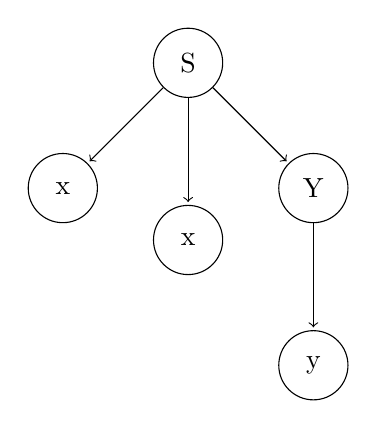
\begin{tikzpicture}[shorten >=1pt,node distance=2.25cm,on grid,auto]
\node[state] (S) {S};
\node[state] (x1) [below left=of S] {x};
\node[state] (x2) [below=of S] {x};
\node[state] (Y) [below right=of S] {Y};
\node[state] (y) [below=of Y] {y};
\path[->]
(S) edge node {} (x1) edge node {} (x2) edge node {} (Y)
(Y) edge node {} (y);
\end{tikzpicture} \\
Since "xxy" has two different left-most derivations, G is ambiguous. \\

\subsection*{c.}
L = $\lbrace$ x$^i$y$^i$z$^i$: i$\geq$0 $\rbrace$ is can be recognized by M, but not recognized by N. \\
Because it is well known that L is not context free, it cannot be recognized by N(1 stack PDA). \\
However L can be recognized by M(2 stack PDA) and it can be seen below. \\
$\Rightarrow$ Push all initial "x"s to a stack. Push the following "y"s to the other stack. \\
When a "z" is read, pop one "x" and one "y" from the stacks. \\
Since there is a "x" and a "y" for each "z", when the inputs end and the two stacks be empty, it will be accepted. \\
\\
It can be seen that M is at least powerful as N, because a 2 stack PDA can simulate a
1 stack PDA, by not using it's second stack. \\
And, above, we saw that L = $\lbrace$ x$^i$y$^i$z$^i$: i$\geq$0 $\rbrace$ is recognized by M, but not recognized by N. \\
That means, M(a 2 stack PDA) can recognize every language which N(a 1 stack PDA) can recognize, also M can recognize at least one different language(L) that cannot be recognized by N. \\
So, M is more powerful than N. \\

\end{document}

​

